\begin{figure}[pos=t]
    \centering
    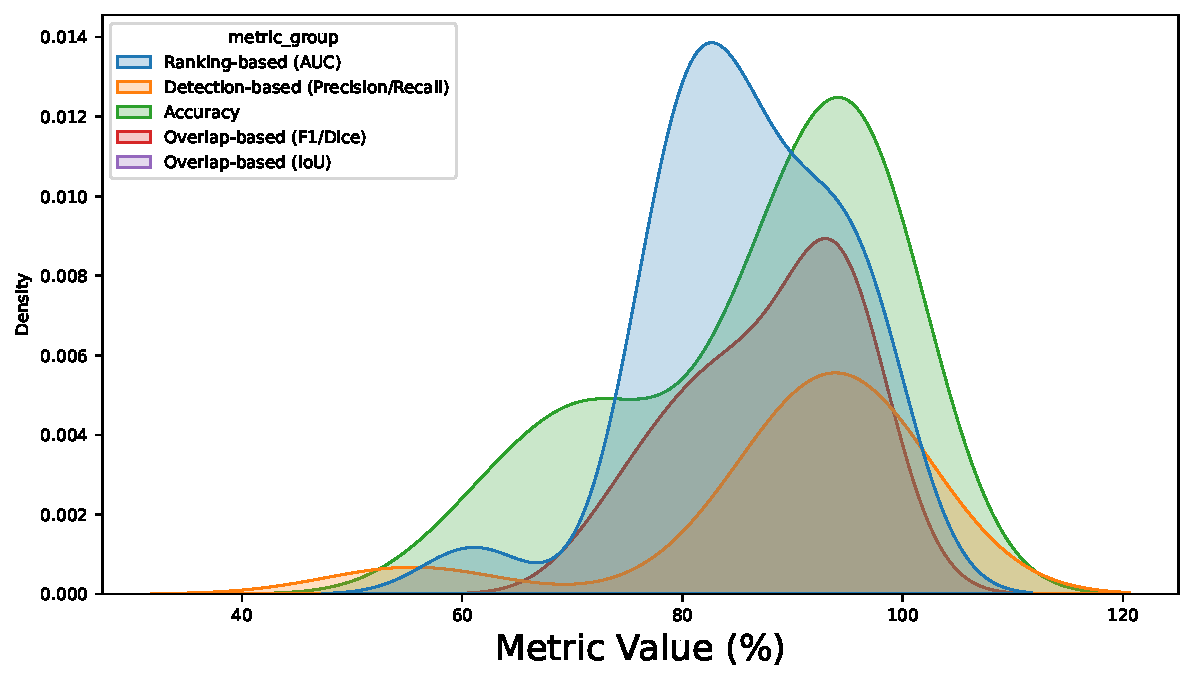
\includegraphics[width=1\linewidth]{kde_metrics.pdf}
    \caption{Kernel density estimates of primary performance metric values, normalised to a 0--100 scale and stratified by metric family. Accuracy values (orange) exhibit the narrowest, highest-peaked distribution centred near 95\%, consistent with binary or near-balanced classification tasks where high accuracy is achievable but potentially misleading under class imbalance. Overlap-based F1/Dice values (blue) and ranking-based AUC values (green) show broader distributions centred near 75--85\%, reflecting the greater difficulty of dense prediction and ranking tasks. IoU (red) is the flattest and lowest-centred distribution, consistent with its known pessimistic bias relative to Dice for the same underlying predictions.}
    \label{fig:metric_kde}
\end{figure}
